\section{Merge Sort}
\label{sec:merge_sort}


\begin{frame}
	\frametitle{Merge Sort}
	\framesubtitle{XKCD Ineffective Sorts: \url{https://xkcd.com/1185/}}
	\begin{center}
		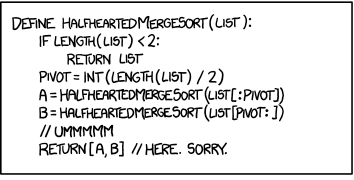
\includegraphics[width=0.8\textwidth]{figures/mergesort.png}\\
	\end{center}
\end{frame}

\begin{frame}
	\frametitle{Merge Sort}
	\begin{block}{Merge Sort}
		A recursive sorting algorithm.\\
		\pause
		It splits the list into two, sorts each half, then combines the results.
	\end{block}	
	\pause
	\begin{alertblock}{Not great for humans}
		As you discovered yesterday, this algorithm is not the easiest for humans to perform.
	\end{alertblock}	
	\pause
	\begin{exampleblock}{Great for computers}
		But computers do excellent at it!
	\end{exampleblock}	
\end{frame}

\begin{frame}
	\frametitle{The idea}
	\begin{overlayarea}{\textwidth}{\textheight}
		\begin{columns}
			\column{0.705\textwidth}
			The algorithm:
		\begin{algorithmic}
			\scriptsize
			\Function{MergeSort}{xs}
			\If{len(xs) $< 2$}	
			\State \Return xs
			\EndIf
			\pause
			\State leftHalf $\gets$ \Call{MergeSort}{the first half of the list}
			\State rightHalf $\gets$ \Call{MergeSort}{the second half of the list}
			\pause
			\State result $\gets []$, $i \gets 0$, $j \gets 0$
			\While{$i < $ len(leftHalf) and $j < $ len(rightHalf)}
			\only<3>{
				\dots
			}
			\only<4>{
			\State\alert{Something goes here}
			\State\alert{Update $i$ and $j$ accordingly.}
		}
		\only<5->{
			\If{leftHalf[i] $<$ rightHalf[j]}
			\State result.append(leftHalf[i]),  $i\gets i + 1$
			\Else
		}
		\only<5>{
			\State 
		}
		\only<6->{
			\State result.append(rightHalf[j]),  $j\gets j + 1$
		}
		\only<5->{
			\EndIf
		}
			\EndWhile
			\only<7>{
				\State \alert{Something here?}
			}
			\only<8->{
				\tiny
			\While{$i < $ len(leftHalf)}
			\State result.append(leftHalf[i]),  $i\gets i + 1$
			\EndWhile
			\While{$j < $ len(rightHalf)}
			\State result.append(rightHalf[j]),  $j\gets j + 1$
			\EndWhile
		}
		\scriptsize
		\State \Return result
			\EndFunction
		\end{algorithmic}
		
			\column{0.305\textwidth}
			\only<4>{
			\begin{questionblock}{What do we do here?}
				\begin{enumerate}[A.]
					\item Compare leftHalf[0] with rightHalf[0]
					\item Compare leftHalf[i] with rightHalf[0]
					\item Compare leftHalf[0] with rightHalf[j]
					\item Compare leftHalf[i] with rightHalf[j]
				\end{enumerate}
			\end{questionblock}
				}
			\only<7>{
			\begin{questionblock}{What do we do here?}
				\begin{enumerate}[A.]
					\item Nothing, we're done
					\item Empty the remainder of the left half, then the right half.
					\item Empty the remainder of the right half, then the left half.
					\item Only one half can still have items left, empty that one.
				\end{enumerate}
			\end{questionblock}
				}
			\only<9->{
				\begin{alertblock}{You can see one con}
					The algorithm is a bit more involved...
			\end{alertblock}
				}
			\only<10->{
				\begin{questionblock}{Is it better?}
					What is a tight bound on the run time?\\
					Hint: you can use the master theorem!
			\end{questionblock}
				}
		\end{columns}
	\end{overlayarea}
\end{frame}

\begin{frame}
	\frametitle{Merge sort run time}
	\begin{answerblock}{Run time}
		$T(0) = T(1) = c_0$ and $T(n) = 2T(n/2) + \Theta(n)$.\\
		This gives $n^{\log_2(2)} = n$ leaves, and as $f(n) = \Theta(n)$ this makes this case 2 of the master method.\\
		Thus $\Theta(n\log n)$ work! We improved!
	\end{answerblock}

	\pause
	\begin{questionblock}{Worst-case instance?}
		What would be the worst type of list for this algorithm?
	\end{questionblock}
	\pause
	\begin{answerblock}{There is none}
		There is no worst-case instance, all of them take $\Theta(n \log n)$ time as we append $n$ items in $\log n$
		recursive calls in the recursion tree.
	\end{answerblock}
\end{frame}

\begin{frame}
	\frametitle{Let's do one example!}
	\begin{block}{But on the smartboard}
		Making this in Tikz is way too much effort ;)
	\end{block}		
\end{frame}

\begin{frame}
	\frametitle{Merge sort: pros and cons}
	\begin{block}{Merge sort}
			Recursively split the list, sort and merge sorted lists.
		\end{block}	
		\begin{exampleblock}{Pros}
			\begin{itemize}
				\item Great in a distributed setting, as it can be parallelised!
				\item Great time complexity! $O(n\log n)$
			\end{itemize}
		\end{exampleblock}	
		\begin{alertblock}{Cons}
			\begin{itemize}
				\item A bit harder to implement.
				\item Always takes $O(n \log n)$ even when only two items would have to be switched.
			\end{itemize}
		\end{alertblock}	
\end{frame}
